

\subsection{Method}

The GP part of the assignment required one nonlinear model structure to
be fitted and analysed using the measured motor voltage and disk angle
\cite{assignment5sc28}. The angular velocity was therefore not used.
A nonlinear autoregressive model with exogenous input (NARX) was
selected because the delayed input and output samples provide an
input--output representation of the system dynamics without requiring
an explicit state estimate.

The NARX regressor is defined as

\begin{equation}
\begin{aligned}
\mathbf{x}(k) =
\big[&
u(k-n_b),\ldots,u(k-1),\\
&
\theta(k-n_a),\ldots,\theta(k-1)
\big]^{\top},
\end{aligned}
\label{eq:gp_regressor}
\end{equation}

where \(n_a\) is the number of delayed angle samples and \(n_b\) is the
number of delayed voltage samples. Because the Mat\'ern-\(5/2\) kernel
is used with automatic relevance determination, each component of
\(\mathbf{x}(k)\) is assigned its own length scale, so the ordering of
the regressor entries does not affect the model. The ordering in
\eqref{eq:gp_regressor} is fixed to match the implementation, so that
the delayed angle \(\theta(k-1)\) occupies the last entry and is used
directly in the angle reconstruction \eqref{eq:gp_angle_reconstruction}.

Instead of predicting the absolute angle directly, the final model
predicts the angle increment

\begin{equation}
\Delta\theta(k)=\theta(k)-\theta(k-1).
\label{eq:gp_delta_target}
\end{equation}

The GP-NARX model is therefore written as

\begin{equation}
\Delta\theta(k)
=
f_{\mathrm{GP}}\!\left(\mathbf{x}(k)\right)+e(k),
\label{eq:gp_delta_model}
\end{equation}

and the predicted angle is reconstructed using

\begin{equation}
\hat{\theta}(k)
=
\theta(k-1)+\widehat{\Delta\theta}(k).
\label{eq:gp_angle_reconstruction}
\end{equation}

The delta-output formulation was used because the change in angle
between two consecutive samples is smaller and smoother than the
absolute angle. The GP therefore models the local system evolution
instead of the complete angle signal. In the experiments, this reduced
the recursive simulation error compared with direct angle prediction.

A Gaussian Process defines a probability distribution over possible
nonlinear functions \cite{course5sc28}. For the model in
\eqref{eq:gp_delta_model}, the unknown function is assigned the prior

\begin{equation}
f_{\mathrm{GP}}(\mathbf{x})
\sim
\mathcal{GP}\!\left(0,k(\mathbf{x},\mathbf{x}')\right),
\end{equation}

where \(k(\mathbf{x},\mathbf{x}')\) is the covariance kernel. Given the
training inputs \(\mathbf{X}\) and targets \(\mathbf{y}\), conditioning
this prior on the data yields a Gaussian predictive distribution
\cite{course5sc28}. The predictive mean at a new regressor
\(\mathbf{x}_{*}\) is

\begin{equation}
\hat{f}(\mathbf{x}_{*})
=
\mathbf{k}_{*}^{\top}
\left(
\mathbf{K}+\sigma_n^2\mathbf{I}
\right)^{-1}
\mathbf{y},
\label{eq:gp_mean}
\end{equation}

while the predictive variance is

\begin{equation}
\hat{\sigma}_{f}^{2}(\mathbf{x}_{*})
=
k(\mathbf{x}_{*},\mathbf{x}_{*})
-
\mathbf{k}_{*}^{\top}
\left(
\mathbf{K}+\sigma_n^2\mathbf{I}
\right)^{-1}
\mathbf{k}_{*}.
\label{eq:gp_variance}
\end{equation}

Equations \eqref{eq:gp_mean}--\eqref{eq:gp_variance} are the full GP
predictive mean and variance \cite{course5sc28}. The predictive mean is
used as the model output, while the predictive variance represents the
remaining model uncertainty. The predictive mean can equivalently be
written as

\begin{equation}
\hat{f}(\cdot)
=
\sum_i \hat{\alpha}_i\,k(\cdot,\mathbf{x}_i),
\qquad
\hat{\boldsymbol{\alpha}}
=
\left(\mathbf{K}+\sigma_n^2\mathbf{I}\right)^{-1}\mathbf{y}.
\label{eq:gp_kernel_expansion}
\end{equation}

This is the core GP estimator. The kernel hyperparameters (the ARD
length scales and the kernel variance) together with the Gaussian noise
variance \(\sigma_n^2\) were estimated from the training data by
minimizing the negative log marginal likelihood
\begin{equation}
\begin{aligned}
-\log p(\mathbf{y}\mid\mathbf{X},\boldsymbol{\eta})
={}& \tfrac{N}{2}\log 2\pi
+ \underbrace{\tfrac{1}{2}\mathbf{y}^{\top}\!\left(\mathbf{K}+\sigma_n^2\mathbf{I}\right)^{-1}\!\mathbf{y}}_{\text{data-fit term}}\\
&+ \underbrace{\tfrac{1}{2}\log\det\!\left(\mathbf{K}+\sigma_n^2\mathbf{I}\right)}_{\text{complexity term}}.
\end{aligned}
\label{eq:gp_marglik}
\end{equation}

which automatically trades off a data-fit term against a
model-complexity term \cite{course5sc28}. In the implementation this
objective was minimized with the L-BFGS-B optimizer using its analytic
gradient.

The regressors and target values were normalized before training.
After constructing the delayed regressors, the available records
contained \(24490\) training samples and \(10490\) validation samples.
The temporal order of the data was preserved, since random shuffling of
individual time samples would not provide a realistic free-run
simulation test.

Preliminary GP experiments compared several kernels using the same
initial direct-output NARX structure. These early tests were used only
to choose a reasonable kernel before the final sparse delta-output GP
was trained. The results are shown in
Table~\ref{tab:gp_kernel_comparison}.

\begin{table}[htbp]
\caption{Initial GP kernel comparison on the validation data.}
\centering
\begin{tabular}{lc}
\toprule
Kernel & Prediction RMSE \\
\midrule
RBF & 0.3583 deg \\
Mat\'ern-\(3/2\) & 0.2514 deg \\
Linear + RBF & 0.2515 deg \\
Mat\'ern-\(5/2\) & 0.2147 deg \\
\bottomrule
\end{tabular}
\label{tab:gp_kernel_comparison}
\end{table}

The Mat\'ern-\(5/2\) kernel gave the lowest validation prediction error
and was therefore selected. Compared with the RBF kernel, the
Mat\'ern-\(5/2\) kernel assumes less restrictive smoothness, which is
useful for modelling nonlinear mechanical dynamics containing friction
and rapidly changing local behaviour. Automatic relevance
determination was used, meaning that each delayed input and output
component had its own length scale.

The lag orders were then varied using

\begin{equation}
n_a\in\{5,8,10\},
\qquad
n_b\in\{5,8\}.
\label{eq:gp_lag_grid}
\end{equation}

In the preliminary lag-order tests, the setting \(n_a=10,n_b=5\)
gave the best first-round one-step prediction result, while the setting
\(n_a=10,n_b=8\) gave the best free-run simulation result among the
tested models. Since the assignment evaluates both prediction and
simulation, the latter configuration was selected. Ten delayed angle
samples provide sufficient output memory, while eight delayed voltage
samples capture the delayed influence of the motor input without making
the regressor unnecessarily large.

A full GP assigns one kernel slice \(k(\cdot,\mathbf{x}_i)\) and one
weight \(\hat{\alpha}_i\) to every training sample, so kernel-matrix
inversion scales as \(\mathcal{O}(N^3)\) and becomes prohibitive for
the \(N=24490\) training samples
\cite{course5sc28}. The full data set was therefore summarized by
\(M\ll N\) inducing points. The \texttt{SparseGPRegression} model in
GPy implements the variational (VFE) sparse approximation, in which the
inducing inputs \(\mathbf{Z}\) together with the kernel and noise
hyperparameters are jointly optimized by maximizing a variational lower
bound on the marginal likelihood \eqref{eq:gp_marglik}. The inducing
points were initialized using MiniBatch \(k\)-means clustering on the
normalized regressors, so that their initial locations covered the
regions with the largest data density. During training, the
inducing-point locations, kernel variance, ARD length scales, and
Gaussian noise variance were further optimized with L-BFGS-B.

Table~\ref{tab:gp_tuning} summarizes the main modelling steps.

\begin{table}[htbp]
\caption{Main GP model tuning steps on the validation data.}
\centering
\begin{tabular}{lcc}
\toprule
Model & Prediction RMSE & Simulation RMSE \\
\midrule
Direct-output GP-NARX & 0.1994 deg & 2.9658 deg \\
Delta-output GP-NARX & 0.1844 deg & 2.5333 deg \\
Sparse delta GP, \(M=150\) & 0.1698 deg & 1.5043 deg \\
Sparse delta GP, \(M=250\) & 0.1638 deg & 1.4615 deg \\
\bottomrule
\end{tabular}
\label{tab:gp_tuning}
\end{table}

The comparison shows that predicting the angle increment improved both
prediction and simulation. Introducing the sparse GP approximation
also allowed all available training samples to be used instead of a
small subset. Increasing the number of inducing points from
\(M=150\) to \(M=250\) gave a further reduction in both errors.
Therefore, \(M=250\) was selected as the final value. This value is
still much smaller than the number of training samples, while providing
the best simulation result among the tested sparse models.

The final model is consequently a sparse delta-output GP-NARX model
with a Mat\'ern-\(5/2\) ARD kernel, \(n_a=10\), \(n_b=8\), and
\(M=250\) inducing points. One-step prediction uses measured past
angles in the regressor, whereas free-run simulation recursively feeds
the previously simulated angles back into the model.


\subsection{GP Results}

Table~\ref{tab:gp_results} summarizes the validation performance of the
final sparse delta-output GP-NARX model. The errors are reported in both
radians and degrees. The final model used \(n_a=10\), \(n_b=8\), a
Mat\'ern-\(5/2\) ARD kernel, and \(M=250\) inducing points.

\begin{table}[htbp]
\caption{Validation results of the final sparse GP model.}
\centering
\begin{tabular}{lcc}
\toprule
Task & RMSE [rad] & RMSE [deg] \\
\midrule
One-step prediction & 0.002859 & 0.1638 \\
Free-run simulation & 0.025508 & 1.4615 \\
\bottomrule
\end{tabular}
\label{tab:gp_results}
\end{table}

The one-step prediction error is considerably smaller than the
simulation error. In the prediction task, the measured past angles are
used to construct the NARX regressor at every sample. Therefore, local
prediction errors do not propagate to later time steps. In the
simulation task, only the initial output history is measured. The GP
then recursively uses its own simulated outputs, so small modelling
errors accumulate over time.

The final simulation normalized root mean squared error was

\begin{equation}
\mathrm{NRMS}_{\mathrm{sim}} = 5.04\%.
\end{equation}

Fig.~\ref{fig:gp_simulation} compares the measured validation output
with the free-run simulation of the final sparse GP model.

\begin{figure}[htbp]
\centerline{
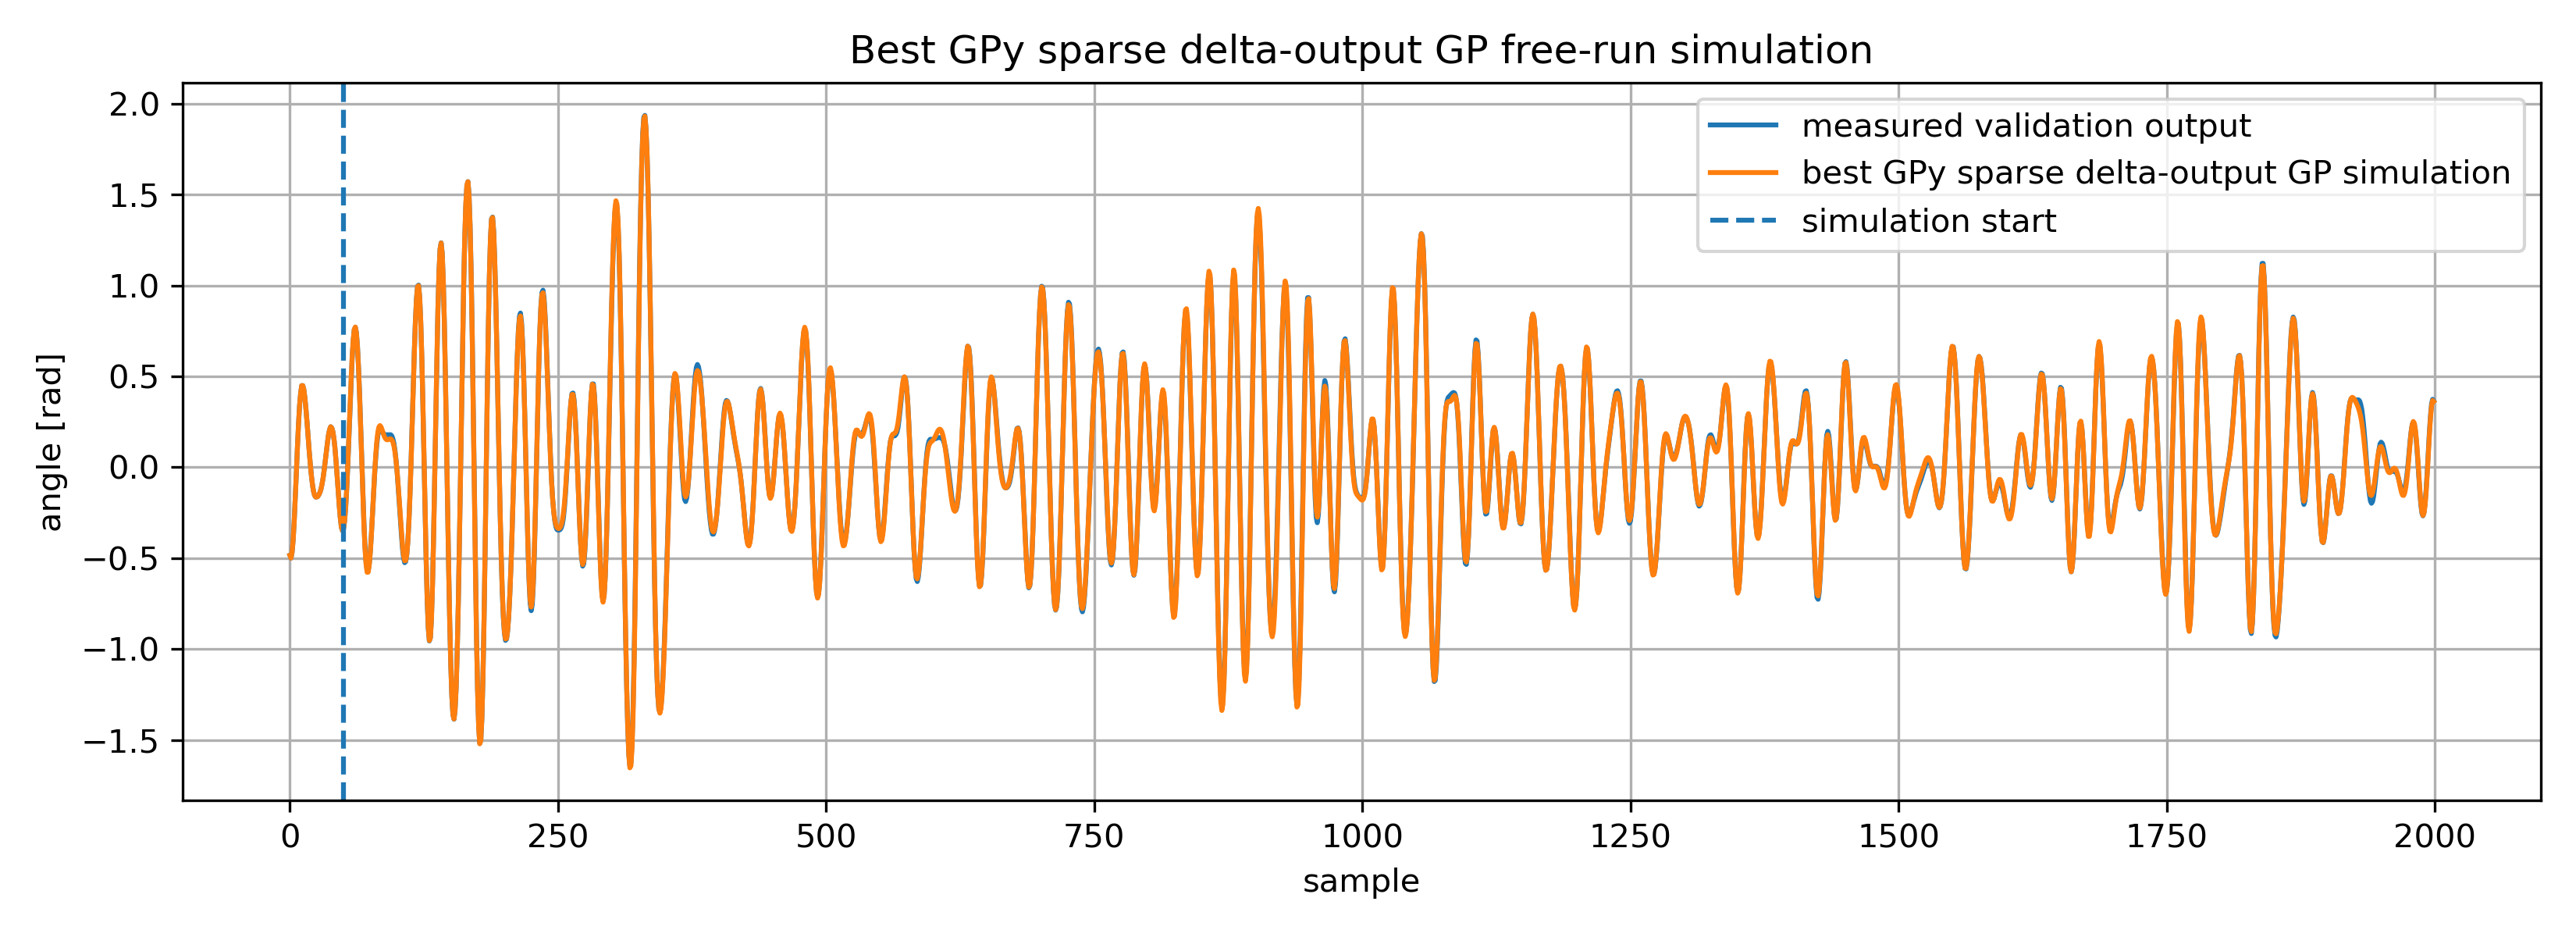
\includegraphics[width=\columnwidth]
{figures/gp_validation_simulation.png}
}
\caption{Measured validation angle and free-run simulation of the final
sparse delta-output GP-NARX model.}
\label{fig:gp_simulation}
\end{figure}

The simulated angle follows the measured output closely over most of
the validation interval. The model reproduces both the oscillation
frequency and the main amplitude variations. This indicates that the
selected delayed angle and voltage samples contain sufficient
information to represent the dominant input--output dynamics of the
disk.

The simulation error is shown in
Fig.~\ref{fig:gp_simulation_error}.

\begin{figure}[htbp]
\centerline{
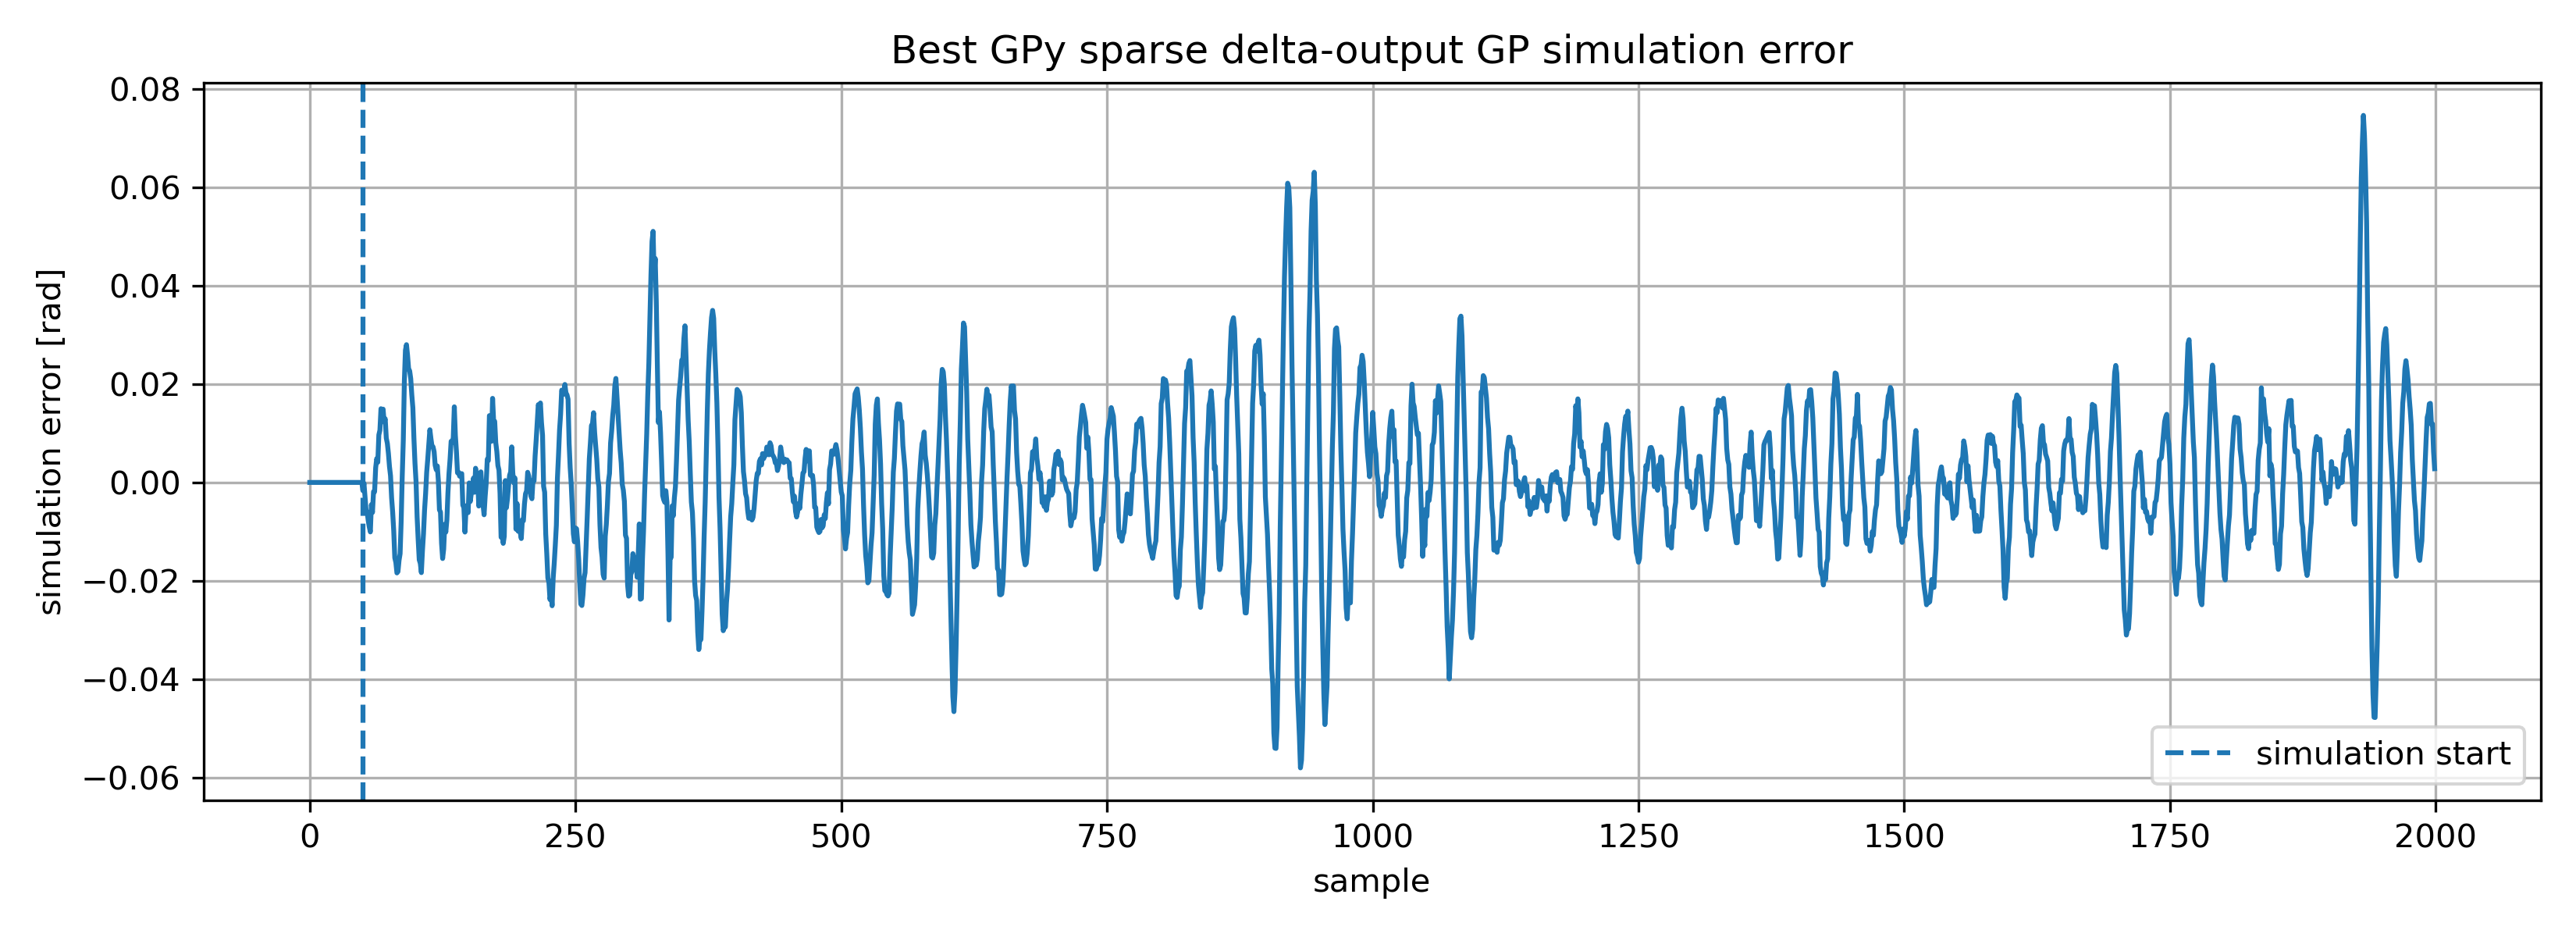
\includegraphics[width=\columnwidth]
{figures/gp_validation_simulation_error.png}
}
\caption{Free-run simulation error of the final sparse delta-output GP
model.}
\label{fig:gp_simulation_error}
\end{figure}

The simulation error remains close to zero for most samples. Larger
error peaks occur mainly during intervals with fast angle changes and
large oscillation amplitudes. These regions are more difficult because
a small error in the predicted angle increment also changes the
regressor used in the next simulation step. The resulting mismatch can
temporarily increase before the simulated trajectory returns close to
the measured trajectory.

The improvement obtained during the modelling procedure can also be
seen from the final results. The initial direct-output GP model had a
simulation RMSE of \(2.9658\) deg. Changing the target to the angle
increment reduced this value to \(2.5333\) deg. The sparse GP with
\(M=150\) inducing points further reduced the simulation RMSE to
\(1.5043\) deg, while increasing the number of inducing points to
\(M=250\) resulted in the final value of \(1.4615\) deg.


\subsection{GP Uncertainty and Optimized Hyperparameters}

Unlike a deterministic regressor, the GP also returns the predictive
variance \eqref{eq:gp_variance}, which provides a direct characterization
of the remaining model uncertainty and the associated \(95\%\)
confidence bound \cite{course5sc28}. The hyperparameters obtained by
minimizing the negative log marginal likelihood \eqref{eq:gp_marglik}
are summarized in Table~\ref{tab:gp_hyperparameters}.

\begin{table}[htbp]
\caption{Optimized hyperparameters of the final sparse GP model
(normalized \(\Delta\theta\) output units).}
\centering
\begin{tabular}{lc}
\toprule
Hyperparameter & Value \\
\midrule
Kernel variance \(\sigma_f^2\)   & \(0.674\) \\
Noise variance \(\sigma_n^2\)    & \(5.15\times 10^{-4}\) \\
ARD length scales                & \(18\) (one per regressor) \\
Inducing points \(M\)            & \(250\) \\
\bottomrule
\end{tabular}
\label{tab:gp_hyperparameters}
\end{table}

The number of ARD length scales is

\begin{equation}
n_a+n_b=18,
\end{equation}

confirming that each delayed angle and voltage sample receives its own length scale.
The very small estimated noise variance shows that the
marginal-likelihood fit attributes almost all of the normalized output
variation to the latent function rather than to measurement noise, i.e.\
a high signal-to-noise fit. This is consistent with the large data-fit
term in \eqref{eq:gp_marglik} and with the small one-step prediction
error in Table~\ref{tab:gp_results}.

The predictive variance \eqref{eq:gp_variance} is, however, the
\emph{one-step} posterior uncertainty evaluated at a deterministic
input. In free-run simulation the regressor itself contains previously
simulated, and therefore uncertain, angles. The implemented simulation
propagates only the predictive mean and feeds it back into the
regressor, so the reported confidence bound is exact for one-step
prediction but underestimates the true simulation uncertainty.
Propagating the full distribution would require evaluating the GP at an
uncertain (Gaussian) input, for example through moment matching
\cite{course5sc28}. This was considered out of scope here, since the
identification benchmark only requires the simulated mean trajectory.


\subsection{GP Discussion}

The final sparse delta-output GP-NARX model gave a one-step prediction
RMSE of \(0.1638\) deg and a free-run simulation RMSE of \(1.4615\) deg.
The larger simulation error is expected because prediction uses measured
past angles at every time step, while simulation recursively feeds the
model's own outputs back into the NARX regressor. Therefore, small local
errors can accumulate during simulation.

The Mat\'ern-\(5/2\) kernel was selected because it gave the best
validation prediction result among the tested kernels. It is less
restrictive than the RBF kernel with respect to function smoothness,
which makes it suitable for mechanical dynamics containing friction and
other locally varying nonlinear effects. The use of automatic relevance
determination also allowed every delayed voltage and angle component to
have a separate length scale. Large length scales indicate that the
corresponding regressor has a relatively small local influence, while
smaller length scales indicate a stronger sensitivity of the GP output.

The delta-output formulation improved both prediction and simulation
compared with direct angle prediction. Instead of learning the complete
angle value, the GP learns the smaller change between two consecutive
samples. This provides a more local representation of the dynamics and
reduces the variation of the regression target. However, recursive
simulation can still drift because an error in one predicted increment
changes the delayed angle values used in the following regressors.

The sparse GP approximation was necessary because a full GP scales
cubically with the number of training samples \cite{course5sc28}.
Using inducing points made it possible to train the model using the full
available training set. The inducing points were initialized using
MiniBatch \(k\)-means clustering, so that they initially represented
regions with a high density of regressors. Their locations and the GP
hyperparameters were then jointly optimized during training by
maximizing the variational bound on the marginal likelihood.

Increasing the number of inducing points from \(M=150\) to \(M=250\)
improved the prediction RMSE from \(0.1698\) deg to \(0.1638\) deg and
the simulation RMSE from \(1.5043\) deg to \(1.4615\) deg. The
improvement was relatively small, but \(M=250\) was selected because it
gave the best simulation result among the tested sparse models.
Simulation performance was given more weight in the final selection
because it evaluates whether the identified model can reproduce the
system dynamics recursively rather than only predict one sample ahead.

The selected lag orders \(n_a=10\) and \(n_b=8\) also represent a
trade-off. A larger number of delayed samples provides more information
about the system memory, but it also increases the regressor dimension
and the number of GP hyperparameters. Among the tested configurations,
this setting gave the best simulation performance without further
increasing the model dimension.

The main limitation is that only a finite set of kernels, lag orders,
and inducing-point counts was tested. A better configuration may
therefore still exist. In addition, the GP is reliable mainly in regions
that are sufficiently represented by the identification data. Since a
kernel model generally interpolates better than it extrapolates, the
prediction uncertainty and error may increase when the model is
evaluated outside the operating range of the training data. As discussed
above, the predictive variance also quantifies this growing uncertainty,
although in free-run simulation only the mean was propagated.

Finally, the true measured outputs for the hidden benchmark tests were
not available during development. Consequently, the final hidden
prediction and simulation files could only be checked for the required
format and dimensions before submission. Their actual performance will
be evaluated by the course staff.
